\documentclass[11pt,a4paper]{article}
\usepackage[margin=2.5cm]{geometry}
\usepackage{amsmath,amssymb}
\usepackage{graphicx}
\usepackage{booktabs}
\usepackage{cite}
\usepackage[hidelinks]{hyperref}

\newcommand{\C}{\mathbb{C}}
\newcommand{\K}{\mathcal{K}}

\title{Quantum Krylov subspace methods\\[2pt]
\large A short note for numerical linear algebraists}
\author{Martin Stoll \and John Pearson}
\date{November 2026}

\begin{document}
\maketitle

\begin{abstract}
Quantum Krylov methods compute the lowest eigenvalue of a huge Hermitian
matrix by running a Rayleigh--Ritz procedure. The quantum computer supplies
the entries of the small projected matrices and a classical computer solves
the resulting generalized eigenvalue problem. This note explains the idea
in standard linear algebra notation. It covers what a quantum device can
and cannot do, which Krylov bases it can generate, and why the main
numerical difficulty is an ill-conditioned Gram matrix whose entries carry
statistical noise. A small experiment illustrates the points, and we list
open questions where numerical linear algebra can contribute.
\end{abstract}

\section{Motivation}

Many problems in quantum physics and chemistry reduce to computing the
smallest eigenvalue $\lambda_0$ of a Hermitian matrix $H \in \C^{n\times n}$.
Physicists call $H$ the \emph{Hamiltonian}, $\lambda_0$ the \emph{ground
state energy} and its eigenvector $u_0$ the \emph{ground state}. For a
system of $N$ particles that each have two possible configurations
(spins, qubits, spin orbitals), $H$ acts on $\C^2\otimes\cdots\otimes\C^2$,
so $n = 2^N$. For
$N=50$, a single vector in double precision already takes 16 petabytes.
Lanczos, Davidson and their relatives are the methods of choice for
moderate $N$. Beyond about $N\approx 50$, any method that stores
vectors explicitly is hopeless, and one turns to compressed formats such
as tensor networks.

A quantum computer with $N$ qubits stores a vector of length $2^N$
\emph{implicitly} and can multiply it by certain unitary matrices
cheaply. The catch is that the vector can never be read out. One only
gets random samples whose statistics encode quadratic forms. Quantum
Krylov methods (also called quantum subspace diagonalization) are
a pragmatic way of combining this ability with the Rayleigh--Ritz
principle \cite{PM19,SHE20,Motta20,Klymko22,CG22,ELN22,Kirby24}. Experiments on current hardware now reach
subspace dimensions and problem sizes of practical interest \cite{Yoshioka25}.
For an NLA reader these methods are attractive because their core
difficulties are classical: a non-orthogonal Krylov basis, an
ill-conditioned Gram matrix, and a generalized eigenvalue problem with
noisy data.

\section{A quantum computer as a restricted linear algebra device}\label{sec:device}

This note assumes no background beyond linear algebra. This section
translates the quantum computing vocabulary into statements about
vectors and matrices. Throughout, $N$ is the number of qubits and
$n=2^N$.

We write $\mathrm{poly}(N)$ for any quantity bounded by $cN^p$ with
constants $c,p$ that do not depend on $N$, such as $2N-1$ or $5N^3$. Since
$N=\log_2n$, this is the same as polylogarithmic in the matrix size $n$,
i.e.\ $O(\log^pn)$, and therefore tiny compared with $n$. By contrast,
$2^N=n$ is \emph{not} $\mathrm{poly}(N)$. ``Efficient'' or ``cheap'' in this note
always means $\mathrm{poly}(N)$. With several arguments, e.g.\
$\mathrm{poly}(N,t,1/\varepsilon)$, the bound is a polynomial in all of
them.

\subsection{Vectors}\label{sec:vectors}

The memory of a quantum computer with $N$ qubits holds a single unit
vector $v\in\C^n$, called the \emph{state}. One qubit holds a unit
vector in $\C^2$, and $N$ qubits hold a vector in
$\C^2\otimes\cdots\otimes\C^2=\C^n$. The standard basis vectors are
indexed by bit strings,
\[
  e_{b_1b_2\dots b_N} = e_{b_1}\otimes e_{b_2}\otimes\cdots\otimes e_{b_N},
  \qquad e_0=\begin{bmatrix}1\\0\end{bmatrix},\; e_1=\begin{bmatrix}0\\1\end{bmatrix},
\]
where each $b_i\in\{0,1\}$ is a binary digit (a \emph{bit}). The bit
string $b=b_1b_2\dots b_N$ is the binary representation of the position
of the entry, counted from $0$. For example, for $N=2$ the vectors
$e_{00},e_{01},e_{10},e_{11}$ are the first to fourth standard basis
vectors of $\C^4$. We identify $b$ with the integer $0,\dots,n-1$ it
represents, so $v_b$ is an entry of $v$. A
\emph{product state} is a Kronecker product $a_1\otimes\cdots\otimes a_N$ of
unit vectors $a_i\in\C^2$. It is described by $2N$ numbers, whereas a
general $v$ needs $n=2^N$. Physicists write $|v\rangle$ for $v$ and
$\langle w|v\rangle$ for $w^*v$. We do not use this notation.

A vector that is \emph{not} a product state is called \emph{entangled}.
In linear algebra terms entanglement is a rank property. For $N=2$,
reshape $v\in\C^4$ into the $2\times2$ matrix
$V=\left[\begin{smallmatrix}v_{00}&v_{01}\\v_{10}&v_{11}\end{smallmatrix}\right]$.
Then $v=a_1\otimes a_2$ holds exactly when $V=a_1a_2^T$, i.e.\ when
$\operatorname{rank}V=1$. For example, $(e_{00}+e_{11})/\sqrt2$ gives
$V=I/\sqrt2$ of rank $2$, so it is entangled. For general $N$, split the
qubits into a first group of $k$ and a second group of $N-k$, and reshape
$v$ into a $2^k\times2^{N-k}$ matrix. Its rank (the \emph{Schmidt rank})
and its singular values (the \emph{Schmidt coefficients}) measure the
entanglement between the two groups. A product state has rank one for
every such split. Vectors with small ranks for the splits $k=1,\dots,N-1$
are exactly those with a cheap tensor-train representation (physicists
call it a \emph{matrix product state}), which is why tensor networks work
well classically for weakly entangled problems. Ground states of many
one-dimensional problems are of this kind, which is why classical
methods such as DMRG succeed there. A generic vector, however, has ranks
growing exponentially in $N$. Many ground states in two and three
dimensions and in chemistry also have large ranks, as do the time-evolved vectors
$e^{-\mathrm{i}tH}v_0$ used below, whose ranks typically grow quickly with $t$.
Storing and manipulating such strongly entangled vectors without writing
them down is what a quantum computer offers.

The device always starts from $e_{0\dots0}$, and all further
vectors are obtained by multiplying with unitary matrices. A start
vector $v_0$ is therefore available only if $v_0=Q_0e_{0\dots0}$ for a
unitary $Q_0$ that can be applied cheaply in the sense of
Section~\ref{sec:unitaries}.

\subsection{Reading out: measurement}\label{sec:measure}

What can be read out of the device shapes everything that follows, so we
discuss it before the computations. On a classical computer the entries
of $v$ sit in memory and can be inspected. On a quantum computer they
cannot. The only way to extract information is a \emph{measurement},
which has three properties a linear algebraist should keep in mind.

\paragraph{1. A measurement returns a random index, not the vector.}
Measuring the state $v$ returns one bit string $b$, chosen at random with
probability
\[
  p_b=|v_b|^2 .
\]
This explains why states are unit vectors: the numbers $|v_b|^2$ are
nonnegative and sum to $\|v\|^2=1$, so they form a probability
distribution on $\{0,\dots,n-1\}$. The vector $v$ is the device's
internal description of this distribution, and we only ever see samples
from it. The device is best thought of as a random number generator
whose distribution we shape by linear algebra (the choice of unitaries)
but whose parameters we cannot read.

\paragraph{2. A measurement destroys the vector.} After the measurement
the state is $e_b$, and $v$ is gone. A second sample requires preparing
$v$ again from $e_{0\dots0}$, i.e.\ running the whole circuit again. One
such run is called a \emph{shot}. A probability $p$ is therefore
estimated as the fraction of $N_s$ shots with the desired outcome. The
standard deviation is $\sqrt{p(1-p)/N_s}\le 1/(2\sqrt{N_s})$, so
accuracy $10^{-3}$ needs on the order of $10^5$--$10^6$ shots. Double
precision is out of reach. Individual entries are hopeless as well: for a
typical $v$ each $p_b$ is about $1/n=2^{-N}$, so one would need about
$2^N$ shots to see a particular $b$ even once. Useful outputs are
therefore a few aggregate numbers, such as the probability of a large
set of outcomes.

\paragraph{3. Phases are invisible.} $v$ and $e^{\mathrm{i}\varphi}v$, or more
generally $v$ and $Dv$ with $D$ a unitary diagonal matrix, give the same
probabilities, because only the moduli $|v_b|$ enter. The information we
want, however, is phase information: eigenvalues appear as phases
$e^{-\mathrm{i}\lambda t}$, and we need inner products $v^*Wv$. The remedy is
\emph{interference}. Add two vectors so that their relative phase changes
the norm of the sum, e.g.\ $\|v+Wv\|^2=2+2\operatorname{Re}(v^*Wv)$ for unitary $W$.
Sections~\ref{sec:unitaries} and~\ref{sec:output} show how the device
does this.

\paragraph{Measuring some of the qubits.} Often only a few qubits are
measured, typically extra qubits added for the purpose. Measuring the
first qubit splits the vector into its two halves $x=[x_0;x_1]$ (here
and below $[x;y]$ denotes the vector with block $x$ on top of block $y$), where
$x_0$ holds the entries whose first bit is $0$ and $x_1$ those whose
first bit is $1$. The outcome $0$ has probability $\|x_0\|^2$, and
afterwards the state is $[x_0;0]/\|x_0\|$. The outcome $1$ has
probability $\|x_1\|^2$, and the state becomes $[0;x_1]/\|x_1\|$. In
linear algebra terms, the measurement applies one of the two orthogonal
projectors $\operatorname{diag}(I,0)$ and $\operatorname{diag}(0,I)$, chosen at
random with probability equal to the squared norm of the projected
vector, and then normalizes. This is the only non-unitary operation
available. It is the mechanism behind the two constructions used
throughout the note:
\begin{itemize}
\item to \emph{estimate a number}, arrange by unitaries that it equals the
  squared norm of a block, then measure (the Hadamard test,
  Section~\ref{sec:output});
\item to \emph{apply a non-unitary matrix} $A$, arrange that $Av$ appears
  in a block, then measure and keep the run only if this block was
  selected (block encodings, Section~\ref{sec:unitaries}).
\end{itemize}

\subsection{The matrix}\label{sec:matrix}

The $n\times n$ matrix $H$ is never stored. It is given as a sum of
$L=\mathrm{poly}(N)$ \emph{Pauli strings} (for the Ising chain below, $L=2N-1$),
\begin{equation}\label{eq:pauli}
  H = \sum_{\ell=1}^{L} \alpha_\ell P_\ell,\qquad
  P_\ell = \sigma_{\ell,1}\otimes\cdots\otimes\sigma_{\ell,N},
\end{equation}
where $\alpha_\ell\in\mathbb{R}$. Each term $P_\ell$ is a Kronecker product of
$N$ matrices of size $2\times2$, one per qubit. The factor
$\sigma_{\ell,i}$ is the one in position $i$ of the $\ell$-th term, and
each factor is one of the four matrices
\[
  I,\quad
  X=\begin{bmatrix}0&1\\1&0\end{bmatrix},\quad
  Y=\begin{bmatrix}0&-\mathrm{i}\\ \mathrm{i}&0\end{bmatrix},\quad
  Z=\begin{bmatrix}1&0\\0&-1\end{bmatrix}
\]
(the \emph{Pauli matrices}). For example, with $N=4$ the string
$P=Z\otimes Z\otimes I\otimes I$ has $\sigma_1=\sigma_2=Z$ and
$\sigma_3=\sigma_4=I$. The $4^N$ Pauli strings form an orthogonal basis of
$\C^{n\times n}$ with respect to $\langle A,B\rangle=\operatorname{trace}(A^*B)$, so
every matrix can be written in the form~\eqref{eq:pauli}. The point is
that physically relevant $H$ need only $L=\mathrm{poly}(N)$ terms, because
most factors are $I$. Each term is stored as its coefficient $\alpha_\ell$
and a word of length $N$ over the alphabet $\{I,X,Y,Z\}$, so storing $H$
needs only $O(LN)$ numbers. Each $P_\ell$ is Hermitian and
unitary. A standard example, used below, is the transverse-field Ising
chain (a simple model of interacting magnetic moments)
\[
  H = -\sum_{i=1}^{N-1} Z_iZ_{i+1} - h\sum_{i=1}^N X_i,
  \qquad Z_i = I\otimes\cdots\otimes I\otimes Z\otimes I\otimes\cdots\otimes I
  \ (Z \text{ in position } i),
\]
and $X_i$ is defined in the same way. $H$ is not unitary, so it cannot
be applied directly. Section~\ref{sec:unitaries} explains what can be
applied instead.

\subsection{Which unitary matrices can be applied}\label{sec:unitaries}

\paragraph{Gates and circuits.} The hardware applies a small set of
elementary unitaries, the \emph{gates}. A one-qubit gate is
\[
  I_{2^{i-1}}\otimes u\otimes I_{2^{N-i}},\qquad u\in\C^{2\times2}\ \text{unitary},
\]
i.e.\ it acts on the $i$-th Kronecker factor only. A two-qubit gate
acts on two neighbouring factors $i,i+1$,
\[
  I_{2^{i-1}}\otimes w\otimes I_{2^{N-i-1}},\qquad w\in\C^{4\times4}\ \text{unitary}.
\]
Applying one gate takes a fixed physical time, independent of $n$. The
device thus performs a ``matvec'' with a $2^N\times 2^N$ matrix in one
step, but only for these very special matrices. A \emph{circuit} is a
product
\[
  Q=\Gamma_q\cdots\Gamma_2\Gamma_1,
\]
where each $\Gamma_j\in\C^{n\times n}$ is a one- or two-qubit gate of the form
above, with its own position $i$ and its own small unitary $u$ or $w$.
$\Gamma_1$ is applied first. The cost of the circuit is the number $q$ of
gates. Gates acting on disjoint factors commute; for example
$(u\otimes I)(I\otimes u')=(I\otimes u')(u\otimes I)=u\otimes u'$. Such gates can
be applied simultaneously. The number of such parallel layers is the \emph{depth},
which determines the run time.

An important construction is the \emph{controlled} version of a unitary
$U\in\C^{n\times n}$,
\begin{equation}\label{eq:controlled}
  C(U) = \begin{bmatrix} I_n & 0\\ 0 & U\end{bmatrix}
  = e_0e_0^T\otimes I_n + e_1e_1^T\otimes U \in \C^{2n\times 2n}.
\end{equation}
It uses one extra qubit (the first Kronecker factor) and applies $U$ to
the lower half of the vector only: $C(U)[x;y]=[x;Uy]$. If $U$ has a circuit, $C(U)$ has one
with a constant factor more gates. The simplest example is the
permutation matrix $C(X)\in\C^{4\times4}$ (the CNOT gate).

\paragraph{Why controlled unitaries matter.} Applying $U$ to $v$ and
measuring reveals only the numbers $|(Uv)_b|^2$ (Section~\ref{sec:measure}, point~3).
Inner products such as $v^*Uv$, and in particular phases, cannot be seen
this way. If $v$ is an eigenvector, $Uv=e^{-\mathrm{i}\varphi}v$, then measuring
$Uv$ gives exactly the same probabilities as measuring $v$. The phase
$\varphi$, which carries the eigenvalue we are after, is invisible. A
phase only becomes visible \emph{relative} to a vector that did not
receive it, and $C(U)$ produces such a pair inside one vector. With the
$2\times2$ unitary (the \emph{Hadamard gate})
\begin{equation}\label{eq:hadamard}
  h=\frac1{\sqrt2}\begin{bmatrix}1&1\\1&-1\end{bmatrix}
  \qquad\text{one gets}\qquad
  (h\otimes I_n)\,C(U)\,(h\otimes I_n)=\frac12\begin{bmatrix}I+U & I-U\\ I-U & I+U\end{bmatrix}.
\end{equation}
This product of three cheap unitaries contains $\tfrac12(I+U)$ as its
leading block. Applied to $[v;0]$, the top block of the result is
$\tfrac12(v+Uv)$. Its squared norm $\tfrac12\big(1+\operatorname{Re}(v^*Uv)\big)$ is the
probability of measuring $0$ on the extra qubit. In this way $C(U)$
turns an inner product into a measurable probability. This is the
Hadamard test of Section~\ref{sec:output}, and the basis of all
eigenvalue algorithms in this note. For an eigenvector the probability
is $\tfrac12(1+\cos\varphi)$, which reveals $\varphi$; this is also the
starting point of phase estimation.

Controlled unitaries play a second role as well. A circuit cannot branch
on the entries of $v$, so $C(U)$ is the linear-algebra replacement of an
if-statement: apply $U$ to the part of the vector where the extra qubit
is $1$. With several extra qubits,
$\sum_\ell e_\ell e_\ell^T\otimes P_\ell$ applies $P_\ell$ to the $\ell$-th block.
Combined with~\eqref{eq:hadamard}-type mixing of the blocks, this is how
linear combinations $\sum_\ell\alpha_\ell P_\ell$ such as $H$ are block encoded
(see below).

\paragraph{What is cheap.} Every unitary in $\C^{n\times n}$ is a product of
gates. However, a generic unitary needs on the order of $n^2=4^N$ gates,
because the unitary matrices form a set of real dimension $n^2$ and each
gate contributes at most 16 real parameters. ``Can be applied'' therefore
means in practice: a circuit with polynomially many gates in $N$, i.e.\
polylogarithmically many in $n$. These matrices are extremely structured.
They resemble classical fast transforms, but the gap is far larger: the
FFT costs $O(n\log n)$ flops, whereas the corresponding quantum circuit
needs only $O(\log^2 n)$ gates. Table~\ref{tab:unitaries} lists the
families relevant for this note.

\begin{table}[t]
\centering
\small
\renewcommand{\arraystretch}{1.15}
\begin{tabular}{@{}p{4.4cm}p{6.6cm}p{3.6cm}@{}}
\toprule
unitary matrix & remark & cost (gates)\\ \midrule
$u_1\otimes\cdots\otimes u_N$, $u_i\in\C^{2\times 2}$ & one gate per factor; includes all Pauli strings $P_\ell$ & $N$, depth 1\\
$\operatorname{diag}\big(e^{\mathrm{i}\varphi(b)}\big)_b$ & $\varphi$ computable by a short classical (Boolean) circuit & $\mathrm{poly}(N)$\\
permutation $e_b\mapsto e_{\pi(b)}$ & $\pi$ computable by a short classical circuit, e.g.\ $b\mapsto b+1 \bmod n$ & $\mathrm{poly}(N)$\\
$e^{-\mathrm{i}\theta P}$, $P$ a Pauli string & $P=QDQ^*$ with $Q$ a Kronecker product and $D$ diagonal (see text) & $O(N)$\\
unitary DFT matrix $F_n$ & $(F_n)_{jk}=\omega^{jk}/\sqrt n$, $\omega=e^{2\pi\mathrm{i}/n}$ (quantum Fourier transform) & $O(N^2)=O(\log^2n)$\\
$C(U)$ & block diagonal, see~\eqref{eq:controlled} & const $\times$ cost$(U)$\\
$e^{-\mathrm{i}tH}$, $H$ as in~\eqref{eq:pauli} & approximately, by products of $e^{-\mathrm{i}\theta P_\ell}$ (see text) & $\mathrm{poly}(N,t,1/\text{accuracy})$\\
$U^k$ & no shortcut in general & $k\times$ cost$(U)$\\
block encoding of $A$ & non-unitary $A$, applied with probability $<1$ (see text) & depends on $A$\\
\bottomrule
\end{tabular}
\caption{Unitary matrices of size $n=2^N$ that a quantum computer can apply
cheaply.}
\label{tab:unitaries}
\end{table}

\paragraph{Exponentials of Pauli strings.} Each $2\times2$ Pauli matrix is
diagonalized by a fixed $2\times2$ unitary: $X=hZh^*$ and $Y=(sh)Z(sh)^*$
with $h$ from~\eqref{eq:hadamard} and $s=\operatorname{diag}(1,\mathrm{i})$. Hence every Pauli string satisfies
$P=QDQ^*$, where $Q$ is a Kronecker product of $2\times2$ unitaries and
$D$ is a Kronecker product of $I$'s and $Z$'s. $D$ is diagonal with
entries $\pm1$, namely the parity of the bits of $b$ in the positions
where $D$ has a $Z$. Therefore $e^{-\mathrm{i}\theta P}=Qe^{-\mathrm{i}\theta
D}Q^*$, and $e^{-\mathrm{i}\theta D}$ is a diagonal matrix of the type in the
second row of Table~\ref{tab:unitaries}.

\paragraph{Time evolution.} Each single term $e^{-\mathrm{i}t\alpha_\ell P_\ell}$ is cheap, but
the matrices $P_\ell$ do not commute, so
$e^{-\mathrm{i}tH}\neq\prod_\ell e^{-\mathrm{i}t\alpha_\ell P_\ell}$. For two Hermitian
matrices $A,B$ and a step $\delta>0$ one has
\[
  \big\|e^{-\mathrm{i}\delta A}e^{-\mathrm{i}\delta B}-e^{-\mathrm{i}\delta(A+B)}\big\|_2
  \le \tfrac{\delta^2}{2}\,\big\|AB-BA\big\|_2 ,
\]
so splitting the exponential is accurate only for \emph{short} times.
The remedy is to cut $t$ into $r$ steps of length $\delta=t/r$. Since
$e^{-\mathrm{i}tH}=\big(e^{-\mathrm{i}(t/r)H}\big)^r$ exactly, one only has to split each short
step:
\[
  e^{-\mathrm{i}tH}\approx\Big(\prod_{\ell=1}^L e^{-\mathrm{i}(t/r)\alpha_\ell P_\ell}\Big)^r
  \qquad\text{(Lie--Trotter)}.
\]
Each of the $r$ factors has error $O\big((t/r)^2\big)$. For unitaries,
errors add up at most linearly: $\|U_1^r-U_2^r\|_2\le r\,\|U_1-U_2\|_2$
(telescoping sum). The total error is therefore $O(t^2/r)$, with a
constant involving the commutators of the $P_\ell$, and it can be made
small by increasing $r$. The circuit consists of $Lr$ Pauli
exponentials, so accuracy $\varepsilon$ costs $r=O(t^2/\varepsilon)$ steps.
Higher-order product formulas and other
methods reduce the cost to roughly linear in $t$. For a general $H$ the
cost of $e^{-\mathrm{i}tH}$ \emph{must} grow linearly with $t$ (this is the
``no fast-forwarding'' theorem). Classically, $H^k$ or $U^k$ are free once
$H$ is diagonalized; here $U^k$ costs $k$ times as much as $U$. In a
Krylov method, the last basis vector is therefore the most expensive one.

\paragraph{Block encodings: using non-unitary matrices.} A non-unitary
$A\in\C^{n\times n}$ with $\|A\|_2\le\alpha$ can be used through a larger
unitary
\[
  W = \begin{bmatrix} A/\alpha & *\\ * & *\end{bmatrix}\in\C^{2^an\times 2^an},
\]
which needs $a$ extra qubits. The blocks $*$ are whatever makes $W$
unitary. A unitary completion always exists, e.g.\ for $a=1$ and
$B=A/\alpha$ (so $\|B\|_2\le1$)
\[
  W=\begin{bmatrix}B&(I-BB^*)^{1/2}\\(I-B^*B)^{1/2}&-B^*\end{bmatrix}.
\]
So in principle $A$ can be any matrix. In practice, what matters is
whether $W$ has a \emph{short} circuit, and for a generic $A$ it does not.
The completion above involves the dense matrix $(I-BB^*)^{1/2}$. A generic
$A$ has $n^2$ independent entries, and just feeding them into the device
already costs at least $n^2$ operations, which is more than a classical
matvec. Exactly as for unitaries, only structured $A$ can be used
cheaply.

\emph{Example: block encoding of $H$.} For $H=\sum_{\ell=1}^L\alpha_\ell P_\ell$
as in~\eqref{eq:pauli}, take $a=\lceil\log_2L\rceil$ extra qubits,
$\alpha=\sum_\ell|\alpha_\ell|$, and the unit vector
$r=\big(\sqrt{|\alpha_\ell|/\alpha}\big)_{\ell=1}^L\in\C^{2^a}$ (padded with zeros).
Let $R$ be a unitary on $\C^{2^a}$ whose first column is $r$, and let
$S=\sum_\ell e_\ell e_\ell^T\otimes\operatorname{sign}(\alpha_\ell)P_\ell$, with $e_\ell$ the
$\ell$-th standard basis vector of $\C^{2^a}$, be the block diagonal matrix
that applies $\pm P_\ell$ to the $\ell$-th block, a controlled unitary in the
sense of~\eqref{eq:controlled}. Then
the matrix $W=(R^*\otimes I_n)\,S\,(R\otimes I_n)$ has the leading $n\times n$ block
\[
  (r^*\otimes I_n)\,S\,(r\otimes I_n)=\sum_\ell \frac{|\alpha_\ell|}{\alpha}\operatorname{sign}(\alpha_\ell)P_\ell=\frac{H}{\alpha}.
\]
$R$ acts on only $a\approx\log_2L$ qubits and $S$ consists of $L$
controlled Pauli strings, so $W$ costs $\mathrm{poly}(N)$ gates. This is
called the \emph{linear combination of unitaries}.

\emph{Which $A$ are cheap?} The main families are:
(i)~linear combinations $\sum_\ell\alpha_\ell U_\ell$ of unitaries with short
circuits, as just shown, with $\alpha=\sum_\ell|\alpha_\ell|$;
(ii)~sparse matrices with at most $s$ nonzeros per row and column whose
positions and values can be computed from the row index by a short
classical circuit, with $\alpha=s\max_{ij}|a_{ij}|$; and
(iii)~everything obtained from these by products, linear combinations,
Kronecker products and polynomials (below). $A$ need not be Hermitian or
even square; in this note, however, $A=H$ throughout.

The normalization $\alpha$ is not a detail. It may be much larger than
$\|A\|_2$; for example, $\sum_\ell|\alpha_\ell|$ often exceeds $\|H\|_2$
considerably. A large $\alpha$ costs twice. First, the success probability
$\|Av\|^2/\alpha^2$ below becomes small. Second, the eigenvalue gap of
$A/\alpha$ shrinks to $(\lambda_1-\lambda_0)/\alpha$, so polynomial filters in
$A/\alpha$ need a higher degree.

Applying $W$ to $[v;0]$ gives
$[Av/\alpha;\,w]$. Measuring the extra qubits
(Section~\ref{sec:measure}) yields the top block with probability
$\|Av\|^2/\alpha^2$, and the state is then $Av/\|Av\|$. Otherwise the
run is discarded. So $A$ is applied only with some probability, and the
result is always normalized. Products of $W$, $W^*$ and simple diagonal
unitaries give block encodings
\[
  \begin{bmatrix} p(A/\alpha) & *\\ * & *\end{bmatrix}
\]
of polynomials $p$ of degree $d$ with $|p(x)|\le1$ on $[-1,1]$ (for
Hermitian $A$), at the cost of about $d$ applications of
$W$~\cite{GSLW19}. For the Chebyshev polynomials $T_k$ this is
particularly simple.

\emph{Classical analogue.} The idea is the same as embedding a Toeplitz
matrix $T\in\C^{n\times n}$ into a circulant $C\in\C^{2n\times2n}$ with leading block
$T$ for fast matvecs. Pad with zeros, apply the larger and better
structured matrix, and keep the top block: $C[x;0]=[Tx;*]$ just as
$W[v;0]=[Av/\alpha;*]$. In both cases the free blocks $*$ are chosen to make
the large matrix cheap to apply, by the FFT in one case and by a short
circuit in the other. There are three differences.
(i)~Classically one simply discards the bottom block. Here discarding is
a projection, which is not unitary; it is done by measuring the extra
qubits, succeeds only with probability $\|Av\|^2/\alpha^2$, and returns the
normalized vector.
(ii)~The scaling by $\alpha$ is forced by unitarity ($\|W\|_2=1$), whereas a
circulant embedding needs no scaling.
(iii)~Classically $T^kx$ is obtained by embedding and truncating $k$
times. Here powers do not compress: the leading block of $W^2$ is
$B^2$ plus a contribution from the $*$ blocks, not $B^2$. Truncating by
measurement after every step multiplies the success probabilities, which
quickly becomes hopeless. Polynomial methods~\cite{GSLW19} therefore
interleave $W$ with simple reflections that act as a ``coherent''
substitute for the truncation. In operator theory this corresponds to
the difference between a unitary dilation of $B$ and a dilation of
all powers of $B$ (Sz.-Nagy, Egerv\'ary).

\paragraph{What is not possible.}
\begin{itemize}
\item Applying a generic dense unitary, which needs exponentially many gates.
\item Applying $H$, or any non-unitary matrix, deterministically. Block
  encodings apply it only with some probability, and the result is
  normalized.
\item Nonlinear operations on the vector: normalization, Gram--Schmidt,
  dividing by an inner product, or any step whose choice depends on the
  entries of $v$ (other than through measurement).
\item Copying: no unitary $Q$ satisfies $Q(v\otimes e_{0\dots0})=v\otimes v$
  for all $v$, since $v\mapsto v\otimes v$ is not linear (the
  ``no-cloning'' theorem).
\item Reading out $v$. Sections~\ref{sec:measure} and~\ref{sec:output} describe what can be
  extracted.
\end{itemize}

\paragraph{Hardware today.} Each two-qubit gate is faulty with probability
around $10^{-3}$, so circuits with more than about $10^3$--$10^4$
two-qubit gates produce mostly noise. Moreover, gates usually act only on
physically neighbouring qubits. Future \emph{error-corrected} hardware
will store each qubit redundantly in many physical qubits and correct
errors on the fly, which allows much longer circuits at a large overhead
in qubits.

\subsection{Output: estimating inner products}\label{sec:output}

We now combine the pieces. By Section~\ref{sec:measure}, a number can be
read out only if it is the probability of a measurement outcome, i.e.\
the squared norm of a block, and phases must first be converted into
norms by interference.

\paragraph{The Hadamard test} estimates $v^*Wv$ for a unitary $W$ with a
circuit. It uses one extra qubit, so all vectors lie in $\C^{2n}$, and $h$ is
the Hadamard gate from~\eqref{eq:hadamard}. Steps 1--3 apply exactly the product in~\eqref{eq:hadamard}.
\begin{enumerate}
\item Prepare $[v;0]$ and apply $h\otimes I_n$: \quad $\tfrac1{\sqrt2}[v;\,v]$.
\item Apply $C(W)$ from~\eqref{eq:controlled}: \quad $\tfrac1{\sqrt2}[v;\,Wv]$.
\item Apply $h\otimes I_n$: \quad $\tfrac12[v+Wv;\,v-Wv]$.
\item Measure the extra qubit. The outcome is $0$ with probability
  $\tfrac14\|v+Wv\|^2=\tfrac12\big(1+\operatorname{Re}(v^*Wv)\big)$.
\end{enumerate}
With $s=+1$ for outcome $0$ and $s=-1$ for outcome $1$, we get
$\mathbb{E}[s]=\operatorname{Re}(v^*Wv)$. Starting step~2 instead from
$\tfrac1{\sqrt2}[v;\,-\mathrm{i}v]$ gives $\operatorname{Im}(v^*Wv)$. Averaging
$N_s$ runs (\emph{shots}) gives an estimate with standard deviation at
most $N_s^{-1/2}$, so an accuracy of $10^{-3}$ costs about $10^6$ runs.
Hardware errors add further, partly systematic, perturbations. All
quantities needed by the Krylov methods below have the form $v_0^*Wv_0$,
with $W=U^k$ or $W=P_\ell U^k$.

Table~\ref{tab:compare} summarizes the consequences for a Krylov method.
The two key restrictions are that inner products are noisy and that the
vectors \emph{cannot be orthogonalized} on the device, since
Gram--Schmidt needs the vectors themselves (Section~\ref{sec:rr}).

\begin{table}[t]
\centering
\small
\begin{tabular}{@{}lll@{}}
\toprule
 & classical Lanczos & quantum Krylov \\ \midrule
storage of $v$ & explicit, $O(n)$ & implicit, $N=\log_2 n$ qubits\\
basis generator & $v\mapsto Hv$ & $v\mapsto f(H)v$, $f(H)$ unitary or block encoded\\
inner products & exact up to rounding & sampled, error $\sim N_s^{-1/2}$\\
orthogonalization & Gram--Schmidt (Lanczos recurrence) & only via $G$ (CholeskyQR-like) \\
projected problem & tridiagonal $T_m$ & dense pencil $(M,G)$, $G$ ill-conditioned\\
\bottomrule
\end{tabular}
\caption{Lanczos versus quantum Krylov methods.}
\label{tab:compare}
\end{table}

\section{Rayleigh--Ritz with a non-orthogonal basis}\label{sec:rr}

Let $v_0,\dots,v_{m-1}$ be vectors that can be prepared on the device and
let $V = [v_0,\dots,v_{m-1}]\in\C^{n\times m}$. $V$ is never formed. We
only need the $m\times m$ matrices
\begin{equation}\label{eq:GM}
  G = V^*V,\qquad M = V^*HV,\qquad G_{jk} = v_j^*v_k,\quad M_{jk}=v_j^*Hv_k ,
\end{equation}
which the quantum computer estimates entry by entry. A classical
computer then solves the generalized Hermitian eigenvalue problem
\begin{equation}\label{eq:pencil}
  M c = \theta\, G c ,
\end{equation}
and the smallest Ritz value $\theta_{\min}$ approximates $\lambda_0$, with
Ritz vector $Vc$. In exact arithmetic, and with $G$ positive definite,
this is standard Rayleigh--Ritz on $\operatorname{range}(V)$. By
Courant--Fischer, $\theta_{\min}\ge\lambda_0$, and $\theta_{\min}$
decreases monotonically as the subspace grows. Classically one would
orthonormalize $V$ first. Here this is not possible on the vectors
themselves (see below), so~\eqref{eq:pencil} is the generalized
eigenvalue problem in the original, typically very ill-conditioned,
basis. Everything that follows is about which vectors $v_k$ to choose
and how to cope with $G$.

\paragraph{Why not orthogonalize?} Classical Gram--Schmidt works on the
vectors,
\[
  w = v_k-\sum_{j<k}(q_j^*v_k)\,q_j,\qquad q_k = w/\|w\| ,
\]
and each ingredient fails on the device.
\begin{itemize}
\item The coefficients $q_j^*v_k$ are not available inside the device.
  They can only be estimated by repeated measurement
  (Section~\ref{sec:output}), i.e.\ read out as noisy numbers.
\item The map $v_k\mapsto q_k$ depends on $v_k$ itself (through the
  coefficients and the normalization), so it is not multiplication by a
  fixed unitary matrix, which is all the device can do
  (Section~\ref{sec:unitaries}).
\item The memory holds one vector, which cannot be copied. So
  $q_0,\dots,q_{k-1}$ cannot be kept alongside $v_k$ to subtract them.
\end{itemize}
What remains is to orthogonalize \emph{in coefficient space}. Every
orthonormal basis of $\operatorname{range}(V)$ has the form $VR^{-1}$ with an
invertible $R$, and choosing the Cholesky factor $G=R^*R$ turns
\eqref{eq:pencil} into the standard Hermitian problem
$R^{-*}MR^{-1}y=\theta y$. This is exactly the classical CholeskyQR
algorithm: orthogonalization using only the Gram matrix. CholeskyQR is
known to be unstable because $\kappa_2(G)=\kappa_2(V)^2$. Once $\kappa_2(V)^2$
exceeds the inverse accuracy of $G$, the factor $R$ is meaningless.
Classically that accuracy is the unit roundoff $\mathbf u$, but here it
is the noise level $\varepsilon\approx10^{-3}$. Modified Gram--Schmidt and
Householder avoid the squaring by working on the vectors, which is
precisely what the device cannot do. This is the root of the numerical
difficulties in Section~\ref{sec:noisy}.

One can also aim for orthonormal vectors directly. The Lanczos vectors
are $q_k=\pi_k(H)v_0$ for polynomials $\pi_k$ whose coefficients follow
from the moments of Section~\ref{sec:moments}, and with a block encoding
$\pi_k(H)$ can be applied (Section~\ref{sec:unitaries}). However, the
coefficients of $\pi_k$ must first be computed classically from noisy
measured data, which is the same ill-conditioned problem in another
form.

The Ritz vector itself is not available, only its coefficient
vector $c$. Other quantities, such as expectation values $x^*Ax$ of
observables $A$ in the Ritz vector $x=Vc$, require further matrices
$V^*AV$ estimated in the same way.

\section{Krylov bases that a quantum computer can generate}

\subsection{\texorpdfstring{The role of $f(H)$}{The role of f(H)}}\label{sec:f}

A quantum computer cannot apply $H$, so the basis vectors are
$v_k = f_k(H)v_0$ for functions $f_k$ that the device can implement,
typically powers $f_k = f^k$ of one unitary $f(H)$. Here $f(H)$ does
\emph{not} approximate the product $Hv$. It replaces the
matrix--vector product as the operation that \emph{generates the
subspace}, and $H$ itself enters only through the projected matrix
$M=V^*HV$ in~\eqref{eq:GM}. In a Krylov method the matvec only has to
supply new directions rich in the wanted eigenvector. Write
$H=\sum_i\lambda_iu_iu_i^*$ with $\lambda_0\le\lambda_1\le\cdots$ and
$v_0=\sum_i\gamma_iu_i$. Every $f_k(H)$ has the same eigenvectors as $H$,
so
\[
  v_k = f_k(H) v_0 = \sum_i f_k(\lambda_i)\gamma_i u_i ,
\]
and Rayleigh--Ritz with $H$ extracts the eigenvalues from whatever space
the $f_k$ produce. This is the familiar situation of shift-and-invert
Lanczos, where $(H-\sigma I)^{-1}$ builds the space but one wants
eigenvalues of $H$, or of polynomially filtered subspace iteration.
Every vector in the subspace has the form $\phi(H)v_0$ with
$\phi\in\operatorname{span}\{f_0,\dots,f_{m-1}\}$. The quality of the
space is determined by how well this function space contains filters
$\phi$ that are large at $\lambda_0$ and small on the rest of the
spectrum. The choice of the $f_k$ also fixes the structure of $G$ and
$M$, and therefore how many numbers the device has to estimate. The two
main choices behave quite differently.
\begin{itemize}
\item If $f_k$ is a polynomial of degree $k$, e.g.\
  $f_k(\lambda)=T_k(\lambda/\alpha)$ (Section~\ref{sec:cheb}), then
  $\operatorname{range}(V)=\K_m(H,v_0)$ is exactly the Lanczos space,
  only in a different basis.
\item If $f_k(H)=U^k$ with $U=e^{-\mathrm{i}\Delta tH}$
  (Section~\ref{sec:rt}), the space consists of
  trigonometric polynomials in $H$ applied to $v_0$. It is \emph{not}
  the Lanczos space, and $U^kv_0$ is not an approximation of $H^kv_0$.
  The two are related only in the limit $\Delta t\to0$. Since
  $U = I-\mathrm{i}\Delta tH+O(\Delta t^2)$, the scaled differences
  $\Delta t^{-j}(U-I)^jv_0$ tend to $(-\mathrm{i}H)^jv_0$, and
  $\K_m(U,v_0)\to\K_m(H,v_0)$. In this limit the vectors $U^kv_0$
  become nearly identical, so $G$ becomes singular. A practical
  $\Delta t\approx\pi/\|H\|_2$ is therefore a deliberate move away from
  the Lanczos space: one gets a different space, still containing good
  filters, whose basis $U^kv_0$ is far better conditioned than for small
  $\Delta t$ (though still ill-conditioned, see Section~\ref{sec:noisy}).
\end{itemize}

\subsection{Real-time Krylov}\label{sec:rt}

The most popular choice uses powers of the time evolution operator,
\begin{equation}
  v_k = U^k v_0 = e^{-\mathrm{i}k\Delta t H}v_0,\qquad k=0,\dots,m-1,
\end{equation}
i.e.\ $\operatorname{range}(V) = \K_m(U,v_0)$, a Krylov space for the
unitary $U$ rather than for $H$~\cite{PM19,Klymko22,CG22,Kirby24}. Because $U$ is unitary and
commutes with $H$,
\begin{equation}
  G_{jk} = v_0^* U^{k-j} v_0 =: g_{k-j},\qquad
  M_{jk} = v_0^* H U^{k-j} v_0 =: h_{k-j},
\end{equation}
with $g_{-k}=\overline{g_k}$ and $h_{-k}=\overline{h_k}$. Both $G$ and $M$ are
\emph{Hermitian Toeplitz}, so only the $2m$ numbers
$g_0,\dots,g_{m-1}$ and $h_0,\dots,h_{m-1}$ have to be estimated.
$g_k$ is a Hadamard test with $W=U^k$. Using~\eqref{eq:pauli},
$h_k = \sum_\ell \alpha_\ell\, v_0^*P_\ell U^k v_0$ is a weighted sum of
Hadamard tests with $W = P_\ell U^k$.

\paragraph{Spectral picture.} With the eigendecomposition from
Section~\ref{sec:f},
\begin{equation}\label{eq:signal}
  g_k = \sum_i |\gamma_i|^2 z_i^k,\qquad h_k = \sum_i |\gamma_i|^2\lambda_i z_i^k,
  \qquad z_i = e^{-\mathrm{i}\Delta t\lambda_i}.
\end{equation}
The data are samples of a sum of complex exponentials. This connects the
method to Prony's method, matrix pencil methods and filter
diagonalization in signal processing. It also shows
\begin{equation}\label{eq:vandermonde}
  G = Z^* D Z,\qquad Z_{ik} = z_i^k,\quad D=\operatorname{diag}(|\gamma_i|^2),
\end{equation}
so $G$ is a weighted Gram matrix of a Vandermonde matrix with nodes on
the unit circle.

\paragraph{Convergence.} Every vector in the subspace is $p(U)v_0$ for a
polynomial $p$ of degree less than $m$. As for Lanczos, it follows that
\begin{equation}\label{eq:kps}
  \theta_{\min}-\lambda_0 \;\le\;
  (\lambda_{\max}-\lambda_0)\,\frac{1-|\gamma_0|^2}{|\gamma_0|^2}\,
  \min_{\deg p<m}\;\frac{\max_{i\ge1}|p(z_i)|^2}{|p(z_0)|^2}.
\end{equation}
For Lanczos one has $p(\lambda)$ on the real interval
$[\lambda_1,\lambda_{\max}]$ and inserts Chebyshev polynomials
(Kaniel--Paige--Saad). Here $p$ must be small on the arc of the unit
circle containing $z_1,\dots,z_{n-1}$ and large at $z_0$. If
$\Delta t(\lambda_{\max}-\lambda_0)<2\pi$ this arc does not wrap around,
and~\eqref{eq:kps} gives exponential convergence in $m$, with a rate
governed by the angular gap $\Delta t(\lambda_1-\lambda_0)$.
Rigorous versions, including noise, are given in~\cite{ELN22,Kirby24}. The choice of
$\Delta t$ is a trade-off. If it is too large, distinct eigenvalues alias
to the same $z_i$. If it is too small, the nodes cluster and $G$
becomes even more ill-conditioned (this is the Lanczos limit discussed
in Section~\ref{sec:f}). A common choice is
$\Delta t\approx \pi/\|H\|_2$.

The factor $|\gamma_0|^{-2}$ in~\eqref{eq:kps} matters far more than
classically. A random start vector has $|\gamma_0|^2\approx 1/n = 2^{-N}$,
which is useless. One needs a preparable $v_0$ with non-negligible
overlap with the ground state $u_0$. Typical choices are a product state
(Section~\ref{sec:vectors}) or a single standard basis vector $e_b$
selected by a cheap classical approximation (in chemistry the
Hartree--Fock state). This \emph{state preparation} problem is shared by all
quantum eigenvalue algorithms.

\subsection{Chebyshev Krylov via block encodings}\label{sec:cheb}

With a block encoding of $H/\alpha$ one can prepare
$v_k = T_k(H/\alpha)v_0$, and then $\operatorname{range}(V)=\K_m(H,v_0)$
is the \emph{exact} Lanczos subspace~\cite{KMM23}. Only the Chebyshev moments
$\mu_k = v_0^*T_k(H/\alpha)v_0$, $k=0,\dots,2m-1$, are needed, because
$T_jT_k = \tfrac12(T_{j+k}+T_{|j-k|})$ and $xT_k=\tfrac12(T_{k+1}+T_{|k-1|})$ give
\begin{equation}
  G_{jk} = \tfrac12\big(\mu_{j+k}+\mu_{|j-k|}\big),\qquad
  M_{jk} = \tfrac{\alpha}{4}\big(\mu_{j+k+1}+\mu_{|j+k-1|}+\mu_{|j-k|+1}+\mu_{||j-k|-1|}\big),
\end{equation}
i.e.\ Toeplitz-plus-Hankel matrices. Convergence is that of Lanczos, but
block encodings need extra qubits and deeper circuits. This variant
targets future, error-corrected hardware.

\subsection{Unifying view and other variants}\label{sec:moments}

Both variants measure \emph{moments} of the spectral measure
$d\mu(\lambda)=\sum_i|\gamma_i|^2\delta(\lambda-\lambda_i)$ of $H$ with respect to
$v_0$, in the basis $e^{-\mathrm{i}k\Delta t\lambda}$ or $T_k(\lambda/\alpha)$.
Solving~\eqref{eq:pencil} is then the familiar problem of computing
Gauss-type quadrature nodes from (modified) moments~\cite{GM10}. Classically
this is known to be ill-conditioned in the power basis and better
behaved for Chebyshev moments. The quantum setting adds random noise of
size $\varepsilon$ to the moments.

Further variants include imaginary-time bases
$v_k\propto e^{-k\tau H}v_0$ (QLanczos~\cite{Motta20}, where $G$ is Hankel up to diagonal scaling), several
start vectors (block or multireference Krylov~\cite{SHE20}), and
non-Krylov subspaces. Examples are $\operatorname{span}\{v_0,P_1v_0,\dots,P_mv_0\}$
for selected Pauli strings or similar simple matrices
$P_j$~\cite{McClean17}, and spans of standard basis vectors $e_b$ whose
indices $b$ are obtained by measuring a prepared state; in the latter
case $G=I$ and $M$ is computed classically~\cite{RM25}. The common computational core is always the
pencil~\eqref{eq:pencil}.

\section{The numerical core: a noisy, ill-conditioned pencil}\label{sec:noisy}

\paragraph{Ill-conditioning is intrinsic.} The better the space
approximates $u_0$, the closer the basis is to linear dependence.
By~\eqref{eq:vandermonde}, $G$ inherits the exponential
ill-conditioning of Vandermonde matrices with nodes clustered on an arc,
weighted by the possibly tiny $|\gamma_i|^2$. Figure~\ref{fig:exp}
(right) shows $\kappa_2(G)$ growing exponentially until it reaches
$1/\mathbf{u}\approx 10^{16}$ for $m\approx 20$, although $n$ is only $1024$.

\paragraph{Noise.} The device returns $\widetilde G = G+E_G$ and
$\widetilde M = M + E_M$ with $\|E_G\|,\|E_M\|/\|H\|\sim\varepsilon$, and
typically $\varepsilon\in[10^{-4},10^{-2}]$. Once
$\lambda_{\min}(G)\lesssim\varepsilon$, $\widetilde G$ may be indefinite
and the pencil $(\widetilde M,\widetilde G)$ may have eigenvalues far
from the spectrum of $H$, possibly below $\lambda_0$. The variational
guarantee $\theta_{\min}\ge\lambda_0$ is lost. Solving~\eqref{eq:pencil}
naively gives garbage (red curve in Figure~\ref{fig:exp}).

\paragraph{Thresholding.} The standard remedy, known in quantum
chemistry as canonical orthogonalization, is a truncated eigenvalue
decomposition. Compute
$\widetilde G = W\Sigma W^*$, keep the eigenpairs with $\sigma_i>\tau$
(collected in $W_\tau,\Sigma_\tau$), and solve the $r\times r$ standard
Hermitian problem
\begin{equation}\label{eq:thresh}
  \big(\Sigma_\tau^{-1/2}W_\tau^*\,\widetilde M\,W_\tau\Sigma_\tau^{-1/2}\big)\,y = \theta\, y .
\end{equation}
This is the analogue of a truncated SVD for an ill-posed problem, with
$\tau$ a few times the noise level. Why does this work at all when
$\kappa(G)\gg 1/\varepsilon$? Rayleigh--Ritz only needs \emph{one}
good vector in the subspace. If $u_0\approx Vc$ with a coefficient
vector $c$ of moderate norm, the perturbation changes its Rayleigh
quotient by roughly $\varepsilon\|c\|^2$, and thresholding at $\tau$ does
not remove it. Epperly, Lin and Nakatsukasa~\cite{ELN22} turn this argument into a
rigorous stability theory for quantum subspace diagonalization. The
error is bounded by the noiseless Krylov error plus a term controlled by
$\varepsilon$, $\tau$ and the size of good coefficient vectors.
Kirby~\cite{Kirby24} refines the analysis for the real-time basis. In practice, the
achievable accuracy is set by the noise level rather than by $\kappa(G)$.

\paragraph{Experiment.} For Figure~\ref{fig:exp} we take the Ising chain with
$N=10$, $h=1$, the product state $v_0 = 2^{-N/2}(1,\dots,1)^T=a\otimes\cdots\otimes a$
with $a=(1,1)^T/\sqrt2$ as start vector ($|\gamma_0|^2\approx0.47$) and
$\Delta t = \pi/(\lambda_{\max}-\lambda_0)$. Noise is modelled as
independent complex Gaussian perturbations of $g_k$ and $h_k$ with
standard deviations $\varepsilon$ and $\varepsilon\,(\lambda_{\max}-\lambda_0)$,
respectively, with
threshold $\tau=10\varepsilon$ (median over 50 realizations). The
real-time basis converges exponentially, but here more slowly than Lanczos.
Even without noise, rounding limits it to about $10^{-9}$ because
$\kappa(G)\approx10^{16}$. With noise, the error stagnates at roughly
the noise level: about $3\cdot10^{-6}$ for $\varepsilon=10^{-6}$ and
$6\cdot 10^{-4}$ for $\varepsilon=10^{-3}$. Without thresholding there is no
convergence at all.

\begin{figure}[t]
\centering
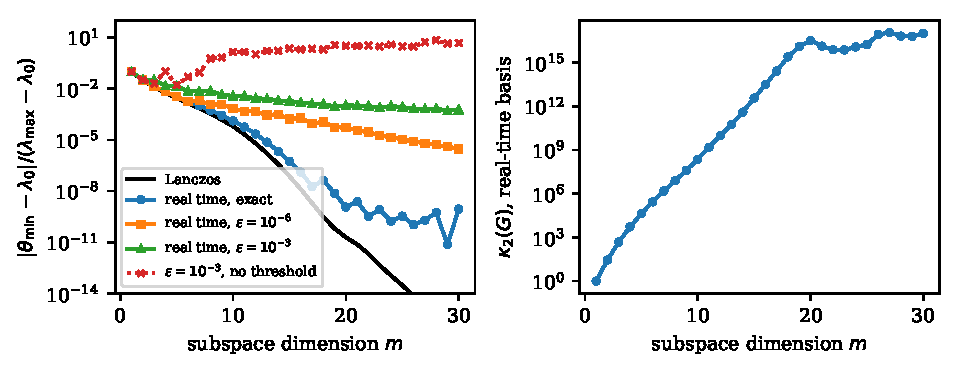
\includegraphics[width=\textwidth]{fig_qk.pdf}
\caption{Ising chain, $n=2^{10}$. Left: relative error of the smallest
Ritz value for Lanczos and for the real-time Krylov method with exact
and noisy matrix elements. Right: condition number of the exact Toeplitz
Gram matrix $G$. Script: \texttt{qk\_experiment.py}.}
\label{fig:exp}
\end{figure}

\section{Cost and practical aspects}

\begin{itemize}
\item \textbf{Shots.} The real-time method needs $O(m)$ distinct numbers.
  Through~\eqref{eq:pauli}, each $h_k$ costs up to $L$ Hadamard tests,
  and each test needs $O(\varepsilon^{-2})$ shots. Grouping commuting
  Pauli strings and tailoring shot budgets to entries reduce this
  (see also Section~\ref{sec:sampling}), but sampling dominates the run
  time.
\item \textbf{Circuit depth.} $v_{m-1}$ requires evolution up to time
  $(m-1)\Delta t$. On noisy hardware the depth limits $m$, which favours
  small subspaces with a good start vector. Trotter errors mean that the
  implemented $U$ commutes with $H$ only approximately, so the Toeplitz
  structure of $M$ is itself an approximation.
\item \textbf{Controlled operations.} The Hadamard test needs
  $C(U^k)$ from~\eqref{eq:controlled}, which is expensive. Variants
  avoid it when an additional vector $r\perp v_0$ with a known eigenvalue
  $Ur=e^{-\mathrm{i}\phi}r$ is available, e.g.\ from a symmetry of $H$;
  superpositions of $v_0$ and $r$ then reveal $v_0^*U^kv_0$ without
  $C(\cdot)$.
\item \textbf{Comparison with phase estimation.} Quantum phase
  estimation, the textbook quantum eigenvalue algorithm, computes $\lambda_0$ to accuracy $\varepsilon$ with evolution
  time $O(1/\varepsilon)$ and needs error-corrected hardware (Section~\ref{sec:unitaries}). Krylov
  methods trade circuit depth for classical post-processing and many
  shots. They are therefore regarded as near-term methods, and they are
  close relatives of recent phase estimation variants designed for the
  first generation of error-corrected hardware, which also process the
  signal $g_k$ classically.
\end{itemize}

\section{Beyond eigenvalues: matrix functions}\label{sec:fun}

Classically, Krylov methods serve matrix functions as much as
eigenvalues. With the Lanczos basis $Q_m$ and the tridiagonal matrix $T_m$,
\[
  v^*f(H)v\approx\|v\|^2e_1^Tf(T_m)e_1,\qquad f(H)v\approx\|v\|\,Q_mf(T_m)e_1 .
\]
The first is Gauss quadrature for the spectral measure, and the second is
the Lanczos approximation~\cite{GM10}. Both carry over to the quantum
setting.

\paragraph{The Krylov approximation in a non-orthogonal basis.} With
$G=R^*R$, the matrix $Q=VR^{-1}$ has orthonormal columns. Since $v_0=Ve_1$,
the Krylov (Galerkin) approximation $Qf(Q^*HQ)Q^*v_0$ can be written using
only the measured matrices:
\begin{equation}\label{eq:fun}
  f(H)v_0\approx V\,f(G^{-1}M)\,e_1,\qquad
  v_0^*f(H)v_0\approx e_1^T\,G\,f(G^{-1}M)\,e_1 .
\end{equation}
Here $G^{-1}M$ is similar to the Hermitian matrix $R^{-*}MR^{-1}$, so $f$ is
evaluated at the Ritz values. In practice one works with the
thresholded matrix of~\eqref{eq:thresh}. For the Chebyshev basis,
\eqref{eq:fun} is Gauss quadrature for the spectral measure $\mu$
(Section~\ref{sec:moments}). For the real-time basis, $\K_m(U,v_0)$ is a
Krylov space of a unitary matrix, and $G$ is a positive definite
Hermitian Toeplitz matrix, namely the moment matrix of the spectral
measure mapped to the unit circle, cf.~\eqref{eq:vandermonde}. The
natural classical tools are then orthogonal polynomials on the unit
circle: the Szeg\H{o} recursion, which is the Levinson algorithm
for $G$, and Szeg\H{o} quadrature, related to the isometric Arnoldi
process~\cite{Gragg93}. These orthogonalize in coefficient space while
exploiting the Toeplitz structure. Their behaviour under measurement
noise is a natural research question. For instance, the recursion
detects loss of positive definiteness of $G$ through reflection
coefficients of modulus at least one.

\paragraph{Linear expansions.} Alternatively, $f$ can be expanded
directly in the functions that are measured,
$f(\lambda)\approx\sum_kc_ke^{-\mathrm{i}k\Delta t\lambda}$ or
$f(\lambda)\approx\sum_kc_kT_k(\lambda/\alpha)$. Then
$v_0^*f(H)v_0\approx\sum_kc_kg_k$ or $\sum_kc_k\mu_k$ is \emph{linear} in the
data. Noise enters only through $\|c\|_1$, and Monte Carlo over $k$
applies (Section~\ref{sec:sampling}). The price is that the expansion is
fixed in advance for the whole spectral interval. In contrast,
\eqref{eq:fun} adapts to the spectrum seen by $v_0$ but is nonlinear in
the noisy data. Classically, this is the same trade-off as between
Chebyshev (kernel polynomial) methods and Lanczos quadrature.

\paragraph{Which functions have been treated.}
\begin{itemize}
\item \emph{Time evolution} $e^{-\mathrm{i}tH}$ beyond the available circuit
  depth. Correlation functions are computed from a Krylov subspace built
  with short evolutions (``fast-forwarding'')~\cite{CDG22}.
\item \emph{Resolvents} $(z-H)^{-1}$, i.e.\ Green's functions. Approaches
  include continued fractions from Lanczos coefficients obtained on a
  quantum computer~\cite{Baker21}, Arnoldi-type methods designed for
  robustness~\cite{NB26}, and Chebyshev expansions with block
  encodings~\cite{Rall20}.
\item \emph{Spectral densities and step functions.} These are treated by
  kernel polynomial expansions~\cite{Rall20} and via the cumulative
  spectral function~\cite{LT22}.
\item \emph{Thermal quantities} with $e^{-\beta H}$. Approaches include
  imaginary-time methods~\cite{Motta20} and Krylov-type methods extended
  to finite temperature~\cite{NB26}.
\end{itemize}
Normalized traces $\frac1n\operatorname{trace}f(H)$, such as the density of
states, are estimated with random start vectors exactly as in
Hutchinson's estimator. This works on hardware~\cite{Summer23} because the
target is $O(1)$, cf.\ Section~\ref{sec:sketch}.

\paragraph{Vectors $f(H)v_0$.} Formula~\eqref{eq:fun} gives only the
coefficient vector $c=f(G^{-1}M)e_1$. As for Ritz vectors, this suffices
for quantities such as $x^*Ax\approx c^*(V^*AV)c$ with $x\approx f(H)v_0$. This
is how correlation functions are obtained in~\cite{CDG22}. Preparing
$f(H)v_0$ itself as a vector on the device from $c$, by a linear
combination of unitaries, succeeds with probability $\|Vc\|^2/\|c\|_1^2$,
which suffers from the ill-conditioning. On error-corrected hardware one
instead applies a fixed polynomial $p\approx f/\max|f|$ through a block
encoding (Section~\ref{sec:unitaries}). The success probability is
$\|p(H/\alpha)v_0\|^2$. Up to logarithmic factors, the degree is about $\alpha t$
for $e^{-\mathrm{i}tH}$, about $\sqrt{\alpha\beta}$ for $e^{-\beta H}$, and about
$\kappa$ for $H^{-1}$, where $1/\kappa$ is the smallest singular value of
$H/\alpha$~\cite{GSLW19}. These polynomials are designed for the whole
interval $[-1,1]$, not for the spectrum seen by $v_0$. The adaptivity
behind the superlinear convergence of classical Krylov methods is
therefore not used. Whether measured moments can be used to design
$v_0$-adapted polynomials that stay bounded on $[-1,1]$ appears to be
open.

\section{Sketching and randomization}\label{sec:sketch}

Randomized numerical linear algebra~\cite{MT20} offers two kinds of
tools. \emph{Sketches} compress a large dimension by a random linear
map. \emph{Monte Carlo sampling} replaces a long sum by a few randomly
chosen terms. In quantum Krylov methods the first kind fails exactly
where it would be most welcome, namely to repair the conditioning of
$G$. The second kind is already central, because on a quantum device the
scarce resources are shots and circuit length, not flops.

\subsection{What does not work: sketching to repair the conditioning}

Classically, sketched Rayleigh--Ritz~\cite{NT24} avoids the squaring of
the condition number in Cholesky\-QR (Section~\ref{sec:rr}). It works
with $SV$ instead of $G=V^*V$, where $S\in\C^{s\times n}$ is random with
$s\approx2m$, and orthogonalizes the small matrix $SV$ by Householder QR.
Since $S$ approximately preserves norms on $\operatorname{range}(V)$, one
has $\kappa(SV)\approx\kappa(V)$, so nothing is squared.

On the device, an entry $s_i^*v_k$ of $SV$ is an inner product. If
$s_i=Q_ie_{0\dots0}$ and $v_k=Q_ke_{0\dots0}$ for unitaries with short circuits, then
$s_i^*v_k=e_{0\dots0}^*(Q_i^*Q_k)e_{0\dots0}$ can be estimated by a Hadamard test
(Section~\ref{sec:output}). Two obstacles appear.
\begin{itemize}
\item \emph{The entries are exponentially small.} For a random unit vector
  $s_i$, $|s_i^*v_k|^2\approx1/n=2^{-N}$, while the device estimates inner
  products only up to an additive error $\varepsilon$
  (Section~\ref{sec:measure}). The rescaling by $\sqrt{n/s}$ that a
  subspace embedding needs amplifies this error by about $2^{N/2}$. This
  is not a weakness of one particular sketch. An \emph{oblivious} sketch,
  i.e.\ one chosen without knowledge of $V$, must work for every
  $m$-dimensional subspace, and for a typical subspace the overlaps with
  any $s$ fixed unit vectors are of size $n^{-1/2}$ (concentration of
  measure).
\item \emph{Random vectors cannot be prepared.} A random unit vector in
  $\C^n$ has no short circuit (Section~\ref{sec:unitaries}).
\end{itemize}
Hadamard probe vectors, as used in diagonal estimation, remove the
second obstacle but not the first. The normalized rows of the
Walsh--Hadamard matrix $F=h\otimes\cdots\otimes h$ are the product states
$Fe_b$, which take $N$ gates. However, they form an orthonormal basis, so
$\sum_b|(Fe_b)^*v|^2=1$ and the typical squared overlap is again $1/n$. A
Hadamard sketch is just a change of basis. It helps only if the Krylov
vectors are concentrated on few rows of $F$, and then measuring $Fv$
samples those rows directly (Section~\ref{sec:sampling}). The subsampled
randomized Hadamard transform is even designed to spread a vector evenly
over all rows, which is exactly the wrong property here. Trace and
diagonal estimation are different: there the target
$\operatorname{trace}(A)/n$ is $O(1)$, so random or Hadamard probes work on a
quantum device too. A Krylov sketch, in contrast, needs $O(1)$ overlaps
with one particular subspace.

A sketch chosen \emph{depending on} $V$ can have $O(1)$ overlaps, e.g.\
$s_i=W_iv_0$ with cheap unitaries $W_i$. Collecting these vectors in
$W=[s_1,\dots,s_s]$, $SV=W^*V$ becomes a cross-Gram matrix, and the pencil
$(W^*HV,W^*V)$ is a Petrov--Galerkin (oblique) projection. In the ideal
case, where $W$ has orthonormal columns and
$\operatorname{range}(V)\subseteq\operatorname{range}(W)$, one has $\|W^*Vx\|=\|Vx\|$ for
all $x$, hence $\kappa(W^*V)=\kappa(V)$ without squaring. But preparing such a
$W$ is the orthogonalization problem again. Whether a well-conditioned,
only approximately suitable $W$ from some other cheap family helps is
open.

\subsection{What does work: sampling}\label{sec:sampling}

\paragraph{Measurement as row sampling.} Measuring a vector $v$ draws a
row index $b$ with probability $|v_b|^2$. In randomized numerical linear
algebra this is squared-row-norm sampling; for a single vector these
are exactly its leverage scores. Sample-based methods use it
directly~\cite{RM25,SKQD}. They measure $v_0$ or the Krylov vectors
$U^kv_0$ many times, collect the set $B$ of observed indices, and solve
the eigenvalue problem for the principal submatrix $H(B,B)$ classically,
e.g.\ by sparse Lanczos. Every Pauli string is a permutation matrix times
a diagonal matrix of phases, so each column of $H$ has at most $L$
nonzeros, which are cheap to compute from~\eqref{eq:pauli}. The basis
$\{e_b\}_{b\in B}$ is orthonormal, so $G=I$ and there is no conditioning
problem. By Cauchy interlacing, $\lambda_{\min}(H(B,B))\ge\lambda_0$ for
every $B$, so noise in the samples only makes the choice of $B$ less
efficient and can never push the result below $\lambda_0$. In NLA terms,
the quantum computer serves as a sampler for column subset selection.

The catch is that $B$ must be manageable, so the ground state has to be
concentrated on relatively few basis vectors. Which basis is right
depends on the problem. For the Ising chain with $N=10$ (script
\texttt{qk\_concentration.py}), the number of basis vectors carrying 99\%
of $\|u_0\|^2$ is 83 in the standard basis versus 467 in the Hadamard
basis for $h=0.5$, and 971 versus 16 for $h=2$. Near the critical value
$h=1$ neither basis works well (793 versus 206 out of $1024$). Under
sparsity assumptions of this kind, polynomial-time convergence has been
proved for the Krylov variant~\cite{SKQD}.

\paragraph{Monte Carlo over sums.} Many quantities have the form
$x=\sum_ic_ix_i$, where each $x_i\in[-1,1]$ can only be sampled, for example
as the mean of a $\pm1$ outcome $s$ of a Hadamard test. Drawing $i$ with
probability $|c_i|/\|c\|_1$ and recording $\|c\|_1\operatorname{sign}(c_i)\,s$ gives an
unbiased estimator of $x$ with variance at most $\|c\|_1^2$. The cost
depends on $\|c\|_1$ and not on the number of terms. This matters when
there are very many or infinitely many terms, and it is the same
principle as in randomized matrix multiplication~\cite{DKM06} and Monte
Carlo trace estimation. Three uses:
\begin{itemize}
\item \emph{Matrix entries.} $h_k=\sum_\ell\alpha_\ell\,v_0^*P_\ell U^kv_0$ costs
  $O(\alpha^2/\varepsilon^2)$ shots with $\alpha=\sum_\ell|\alpha_\ell|$, independently of
  $L$. This matches an optimal distribution of shots over the $L$ terms,
  without enumerating them.
\item \emph{Time evolution (qDRIFT~\cite{Cam19}).} Instead of a
  Lie--Trotter product over all $L$ terms, one multiplies $q$ factors
  $e^{-\mathrm{i}(\alpha t/q)\operatorname{sign}(\alpha_\ell)P_\ell}$, each with $\ell$ drawn with
  probability $|\alpha_\ell|/\alpha$. The circuit length depends on $\alpha$
  and $t$ but not on $L$, which pays off for Hamiltonians with very many
  small terms, as in chemistry. Matrix concentration inequalities show
  that a single random product is already accurate with high
  probability~\cite{CHKT21}, an analysis in the spirit of randomized NLA.
\item \emph{Random times.} If the post-processing is \emph{linear} in the
  signal $g$, one can draw a random time for every shot. Lin and
  Tong~\cite{LT22} estimate the cumulative spectral function
  $x\mapsto\sum_{\lambda_i\le x}|\gamma_i|^2$ in this way; its first jump is at
  $\lambda_0$. Each shot needs a single Hadamard test at one random time.
\end{itemize}
Rayleigh--Ritz, in contrast, is nonlinear in the data, so in Krylov
methods Monte Carlo can only be applied entry by entry.

\paragraph{Randomized measurements.} Classical shadows~\cite{HKP20}
apply a random cheap unitary before measuring, e.g.\ a Kronecker product
of $2\times2$ unitaries drawn from a fixed finite set. From the outcomes
one builds an unbiased random estimate of the rank-one matrix $vv^*$,
the \emph{shadow}. With $O(3^w\log M/\varepsilon^2)$ shots, all $M$ quantities
$v^*Pv$ with Pauli strings $P$ of weight at most $w$ (at most $w$
non-identity factors) are estimated to accuracy $\varepsilon$. The logarithmic
dependence on $M$ is reminiscent of the Johnson--Lindenstrauss lemma.
Off-diagonal quantities $v_j^*Pv_k$ follow in the same way from the vector
$\tfrac1{\sqrt2}[v_j;v_k]$, which uses one extra qubit as in the Hadamard test.
This helps when many different numbers are needed: subspaces spanned by
$P_jv_0$ for many Pauli strings~\cite{BKC24}, or many observables $V^*AV$.
It is less useful for a single sum such as $h_k$, where Monte Carlo over
the terms is simpler.

\paragraph{The classical back end.} In Krylov methods the projected
problems are tiny ($m\lesssim100$), so classical sketching buys nothing
there. Sample-based and shadow-based methods, however, produce large
classical problems: sparse eigenproblems for $H(B,B)$ with very large
$|B|$, or high-dimensional subspace problems~\cite{BKC24}. There,
randomized eigensolvers such as sketched Rayleigh--Ritz~\cite{NT24} apply
directly.

In short, randomization is useful for saving shots and circuit length
and for choosing subspaces. No sketch is known that repairs the
conditioning of the Krylov Gram matrix.

\section{State of the art and open questions}\label{sec:open}

\paragraph{What is established.} The framework of
Sections~\ref{sec:rr}--\ref{sec:noisy} is well understood. Real-time and
Chebyshev bases satisfy Kaniel--Paige--Saad-type convergence
bounds~\cite{ELN22,Kirby24,KMM23}. For the \emph{smallest eigenvalue},
thresholding is stable under small noise: the error is bounded by the
noiseless Krylov error plus a term linear in the noise
level~\cite{Kirby24}, and explicit finite-shot analyses
exist~\cite{LLH24}. Hardware experiments have reached tens of
qubits~\cite{Yoshioka25}, and sampling-based hybrids come with
convergence guarantees under sparsity assumptions~\cite{SKQD}. Almost
everything beyond the smallest eigenvalue under small additive noise is
open. Even there, recent work disagrees on whether ill-conditioning or
statistical noise is the dominant failure mode~\cite{OZG26}. The
following problems seem particularly suited to numerical linear
algebra.

\begin{enumerate}
\item \textbf{Eigenvectors and observables.} The Ritz vector $x=Vc$ is
  only implicit. An observable $x^*Ax$ requires the further matrix
  $V^*AV$, whose noise is amplified by $\|c\|^2$, and $\|c\|$ can be large
  in an ill-conditioned basis. Moreover, observables converge more slowly
  than energies. For $\|x\|=1$ and $\theta=x^*Hx$, one has
  $\sin^2\angle(x,u_0)\le(\theta-\lambda_0)/(\lambda_1-\lambda_0)$, so an energy
  error $\eta$ allows observable errors up to
  $2\|A\|_2\sqrt{\eta/(\lambda_1-\lambda_0)}$. A $\sin\Theta$ theory in the
  sense of Davis and Kahan~\cite{DK70} for noisy, thresholded pencils
  seems to be missing.
\item \textbf{Excited states and spurious eigenvalues.} Thresholding has
  been analysed only for $\lambda_{\min}$. For higher eigenvalues there is no
  comparable theory, and noisy pencils produce spurious Ritz values.
  Recent work proposes filters that detect them~\cite{OZG26}. Lanczos in
  finite precision faces a similar problem, which is handled by the
  Cullum--Willoughby test~\cite{CW85}. An analogue for noisy pencils is
  open.
\item \textbf{Optimal regularization and limits.} Thresholding is a
  heuristic. What are the optimal threshold and regularization, given
  the known covariance of $E_G$ and $E_M$? Can the Toeplitz or Hankel
  structure be preserved, e.g.\ via structured low-rank approximation?
  Equally open is the converse question: what accuracy can be achieved
  at all from $m$ noisy samples $g_k,h_k$? For real-time data this is a
  super-resolution problem, namely estimating the smallest frequency
  in~\eqref{eq:signal}. There, stability limits are understood through
  the conditioning of Vandermonde matrices. Matching them with the
  pencil approach is open.
\item \textbf{A posteriori error estimates.} Classical Krylov methods
  monitor residuals, whereas quantum Krylov methods usually report
  $\theta_{\min}$ without error bars. With $c^*Gc=1$, the residual of the Ritz
  pair satisfies
  \[
    \|Hx-\theta x\|^2=c^*(V^*H^2V)\,c-\theta^2,
  \]
  and $V^*H^2V$ is again Toeplitz for the real-time basis. The residual
  yields the classical residual bound and, given a lower bound on
  $\lambda_1$, Kato--Temple lower bounds on $\lambda_0$~\cite{Parlett98}. How to
  estimate these reliably from noisy data, where the subtraction suffers
  from large $\|c\|$, is open.
\item \textbf{Orthogonal bases on the device.} Orthonormal Lanczos
  vectors $q_k=\pi_k(H)v_0$ can in principle be prepared. One option is to
  apply the Lanczos polynomials through block encodings
  (cf.~\cite{KMM23} and Section~\ref{sec:rr}). Another is an
  operator-level Lanczos recursion, as recently proposed~\cite{OQKD26}.
  Both cost deeper circuits and need recurrence coefficients computed
  from noisy data. This is Lanczos with perturbed coefficients. A theory
  of the resulting loss of orthogonality, in the spirit of Paige's
  analysis of Lanczos in finite precision~\cite{Paige80} with noise
  level $\varepsilon$ in place of $\mathbf u$, would clarify when such schemes beat
  regularized non-orthogonal ones.
\item \textbf{Structured noise.} Most analyses assume small additive
  errors. Real devices add structure. Trotter errors break the
  commutation of $U$ and $H$, and with it the Toeplitz structure of $M$.
  Decoherence damps the signal, roughly $g_k\mapsto f_kg_k$ and
  $h_k\mapsto f_kh_k$ with decaying $f_k$, i.e.\ an entrywise (Hadamard)
  product of $G$ and $M$ with a Toeplitz damping matrix. How such
  structured perturbations move Ritz values, and whether they can be
  undone, has received less attention than additive noise.
\item \textbf{Preparing the Ritz vector.} Many applications need the
  approximate eigenvector \emph{on the device}, e.g.\ as start vector for
  phase estimation. Preparing $x=Vc=\sum_kc_kU^kv_0$ as a linear
  combination of unitaries (Section~\ref{sec:unitaries}) succeeds with
  probability $\|x\|^2/\|c\|_1^2=1/\|c\|_1^2$. This favours coefficient
  vectors with small $\|c\|_1$, i.e.\ a Ritz problem regularized by
  $\|c\|_1$, which trades energy accuracy against preparation cost. We are
  not aware of an analysis of this trade-off.
\item \textbf{Basis design.} Non-uniform time steps, filters, block
  Krylov spaces with several start vectors, hybrid Krylov--sampling
  bases~\cite{SKQD}, and the trade-off between conditioning and aliasing
  in the choice of $\Delta t$.
\item \textbf{Moments, quadrature and matrix functions.} How stable is
  recovering Gauss or Szeg\H{o} quadrature rules from noisy Chebyshev or
  trigonometric moments, e.g.\ via modified moments~\cite{GM10} or the
  Levinson--Szeg\H{o} recursion~\cite{Gragg93}? When is the adaptive but
  nonlinear approximation~\eqref{eq:fun} preferable to fixed linear
  expansions under noise? Can measured moments guide the choice of
  polynomials for block encodings (Section~\ref{sec:fun})?
\item \textbf{Experimental design.} Which entries should be measured,
  and with how many shots, for a given total budget?
\item \textbf{Sketching for conditioning.} Is there a sketch depending on
  $V$ (Section~\ref{sec:sketch}) whose cross-Gram matrix $W^*V$ avoids the
  squaring $\kappa(G)=\kappa(V)^2$ under additive measurement noise? Can
  matrix concentration inequalities give sharp shot counts for the noisy
  pencil?
\item \textbf{Where is the advantage?} All quantum eigenvalue methods
  need a start vector with non-negligible overlap $|\gamma_0|^2$. Whether such
  vectors exist for problems that are hard for classical methods is
  debated~\cite{Lee23}. Fair comparisons with the best classical methods
  are therefore part of the research agenda.
\end{enumerate}

For a broad survey of subspace methods on quantum computers
see~\cite{Motta24}. The analysis in~\cite{ELN22} is written for a
numerical analysis audience and is the natural next read. The list above
reflects the literature as of late 2026 and is not exhaustive.

\small
\begin{thebibliography}{99}
\bibitem{PM19} R.~M. Parrish, P.~L. McMahon, Quantum filter diagonalization:
  quantum eigendecomposition without full quantum phase estimation,
  arXiv:1909.08925, 2019.
\bibitem{SHE20} N.~H. Stair, R.~Huang, F.~A. Evangelista, A multireference
  quantum Krylov algorithm for strongly correlated electrons,
  J.~Chem. Theory Comput.\ 16 (2020), 2236--2245.
\bibitem{Motta20} M.~Motta, C.~Sun, A.~T.~K. Tan, M.~J. O'Rourke, E.~Ye,
  A.~J. Minnich, F.~G.~S.~L. Brand\~ao, G.~K.-L. Chan, Determining eigenstates
  and thermal states on a quantum computer using quantum imaginary time
  evolution, Nature Physics 16 (2020), 205--210.
\bibitem{Klymko22} K.~Klymko et al., Real-time evolution for ultracompact
  Hamiltonian eigenstates on quantum hardware, PRX Quantum 3 (2022), 020323.
\bibitem{CG22} C.~L. Cortes, S.~K. Gray, Quantum Krylov subspace algorithms
  for ground- and excited-state energy estimation, Phys.\ Rev.\ A 105 (2022),
  022417.
\bibitem{ELN22} E.~N. Epperly, L.~Lin, Y.~Nakatsukasa, A theory of quantum
  subspace diagonalization, SIAM J.\ Matrix Anal.\ Appl.\ 43 (2022),
  1263--1290.
\bibitem{Kirby24} W.~Kirby, Analysis of quantum Krylov algorithms with
  errors, Quantum 8 (2024), 1457.
\bibitem{Yoshioka25} N.~Yoshioka et al., Krylov diagonalization of large
  many-body Hamiltonians on a quantum processor, Nature Communications (2025);
  arXiv:2407.14431.
\bibitem{GSLW19} A.~Gily\'en, Y.~Su, G.~H. Low, N.~Wiebe, Quantum singular
  value transformation and beyond, Proc.\ STOC 2019, 193--204.
\bibitem{KMM23} W.~Kirby, M.~Motta, A.~Mezzacapo, Exact and efficient
  Lanczos method on a quantum computer, Quantum 7 (2023), 1018.
\bibitem{GM10} G.~H. Golub, G.~Meurant, Matrices, Moments and Quadrature
  with Applications, Princeton University Press, 2010.
\bibitem{McClean17} J.~R. McClean, M.~E. Kimchi-Schwartz, J.~Carter,
  W.~A. de~Jong, Hybrid quantum-classical hierarchy for mitigation of
  decoherence and determination of excited states, Phys.\ Rev.\ A 95 (2017),
  042308.
\bibitem{RM25} J.~Robledo-Moreno et al., Chemistry beyond the scale of exact
  diagonalization on a quantum-centric supercomputer, Science Advances (2025).
\bibitem{Motta24} M.~Motta et al., Subspace methods for electronic structure
  simulations on quantum computers, Electronic Structure 6 (2024), 013001.
\bibitem{NT24} Y.~Nakatsukasa, J.~A. Tropp, Fast and accurate randomized
  algorithms for linear systems and eigenvalue problems, SIAM J.\ Matrix
  Anal.\ Appl.\ 45 (2024).
\bibitem{HKP20} H.-Y. Huang, R.~Kueng, J.~Preskill, Predicting many
  properties of a quantum system from very few measurements, Nature
  Physics 16 (2020), 1050--1057.
\bibitem{BKC24} G.~Boyd, B.~Koczor, Z.~Cai, High-dimensional subspace
  expansion using classical shadows, arXiv:2406.11533, 2024.
\bibitem{MT20} P.-G. Martinsson, J.~A. Tropp, Randomized numerical linear
  algebra: foundations and algorithms, Acta Numerica 29 (2020), 403--572.
\bibitem{SKQD} Yu, Robledo Moreno, Iosue, et al., Quantum-centric algorithm
  for sample-based Krylov diagonalization, arXiv:2501.09702, 2025.
\bibitem{DKM06} P.~Drineas, R.~Kannan, M.~W. Mahoney, Fast Monte Carlo
  algorithms for matrices I: approximating matrix multiplication, SIAM J.\
  Comput.\ 36 (2006), 132--157.
\bibitem{Cam19} E.~Campbell, Random compiler for fast Hamiltonian
  simulation, Phys.\ Rev.\ Lett.\ 123 (2019), 070503.
\bibitem{CHKT21} C.-F. Chen, H.-Y. Huang, R.~Kueng, J.~A. Tropp,
  Concentration for random product formulas, PRX Quantum 2 (2021), 040305.
\bibitem{LT22} L.~Lin, Y.~Tong, Heisenberg-limited ground-state energy
  estimation for early fault-tolerant quantum computers, PRX Quantum 3
  (2022), 010318.
\bibitem{LLH24} G.~Lee, D.~Lee, J.~Huh, Sampling error analysis in quantum
  Krylov subspace diagonalization, Quantum 8 (2024), 1477.
\bibitem{OZG26} Oliveira, Ziems, Glaser, preprint arXiv:2604.11532, 2026.
\bibitem{DK70} C.~Davis, W.~M. Kahan, The rotation of eigenvectors by a
  perturbation.~III, SIAM J.\ Numer.\ Anal.\ 7 (1970), 1--46.
\bibitem{CW85} J.~K. Cullum, R.~A. Willoughby, Lanczos Algorithms for Large
  Symmetric Eigenvalue Computations, Vol.~I, Birkh\"auser, 1985.
\bibitem{Parlett98} B.~N. Parlett, The Symmetric Eigenvalue Problem, SIAM,
  1998.
\bibitem{OQKD26} Orthogonal quantum Krylov diagonalisation, preprint
  arXiv:2607.09476, 2026.
\bibitem{Paige80} C.~C. Paige, Accuracy and effectiveness of the Lanczos
  algorithm for the symmetric eigenproblem, Linear Algebra Appl.\ 34
  (1980), 235--258.
\bibitem{Lee23} S.~Lee et al., Evaluating the evidence for exponential
  quantum advantage in ground-state quantum chemistry, Nature
  Communications 14 (2023), 1952.
\bibitem{Gragg93} W.~B. Gragg, Positive definite Toeplitz matrices, the
  Arnoldi process for isometric operators, and Gaussian quadrature on the
  unit circle, J.\ Comput.\ Appl.\ Math.\ 46 (1993), 183--198.
\bibitem{CDG22} C.~L. Cortes, A.~E. DePrince~III, S.~K. Gray, Fast-forwarding
  quantum simulation with real-time quantum Krylov subspace algorithms,
  Phys.\ Rev.\ A 106 (2022), 042409.
\bibitem{Baker21} T.~E. Baker, Lanczos recursion on a quantum computer for
  the Green's function and ground state, Phys.\ Rev.\ A 103 (2021), 032404.
\bibitem{NB26} Nelson, Baczewski, Estimating Green's functions with a
  robust quantum Arnoldi method, arXiv:2605.22920, 2026.
\bibitem{Rall20} P.~Rall, Quantum algorithms for estimating physical
  quantities using block encodings, arXiv:2004.06832, 2020.
\bibitem{Summer23} Summer et al., Calculating the many-body density of
  states on a digital quantum computer, arXiv:2303.13476, 2023.
\end{thebibliography}

\end{document}
